\section{Results}\label{sec:results}
\subsection{Primary natural-availability comparison}
Table~\ref{tab:natural} reports replayed natural metrics on the same 9,566 episodes with a fixed support set. AVF attains AUROC 0.7969, macro-F1 0.6194, balanced accuracy 0.6251 and SCR 0.6043. The seed-ensembled LightGBM reference scores 0.7937, 0.6014, 0.5952 and 0.5685. Figure~\ref{fig:performance} highlights the class- and cell-sensitive comparison.
\begin{table}[pos=!ht]
\caption{ROI-only natural evaluation. Values are pooled metrics after averaging three seeds' probabilities per episode. All rows use the same 34 supported cells for SCR. Comparator rows are local adaptations.}\label{tab:natural}
\begin{tabular*}{\tblwidth}{@{} LCCCC @{}}\toprule
Method & AUROC & Macro F1 & BAcc & SCR \\ \midrule
Plain neural & 0.781 & 0.598 & 0.598 & 0.543 \\
+ class weights (CW) & 0.781 & 0.597 & 0.619 & 0.564 \\
+ joint weights (JW) & 0.776 & 0.591 & 0.615 & 0.583 \\
+ modality dropout (MD) & 0.782 & 0.600 & 0.599 & 0.547 \\
+ CW + MD & 0.784 & 0.601 & 0.621 & 0.573 \\
+ JW + MD & 0.778 & 0.593 & 0.621 & 0.585 \\
+ logit adjustment + MD & 0.769 & 0.579 & 0.617 & 0.584 \\
LightGBM seed ensemble & 0.794 & 0.601 & 0.595 & 0.568 \\
TIMM-inspired adaptation & 0.785 & 0.603 & 0.605 & 0.567 \\
Flex-MoE-inspired adaptation & 0.789 & 0.607 & 0.610 & 0.564 \\
UniMIX-inspired adaptation & 0.793 & 0.608 & 0.615 & 0.581 \\
\textbf{AVF (proposed)} & 0.797 & 0.619 & 0.625 & 0.604 \\
\bottomrule\end{tabular*}
\end{table}
\begin{figure}[pos=!ht]
\centering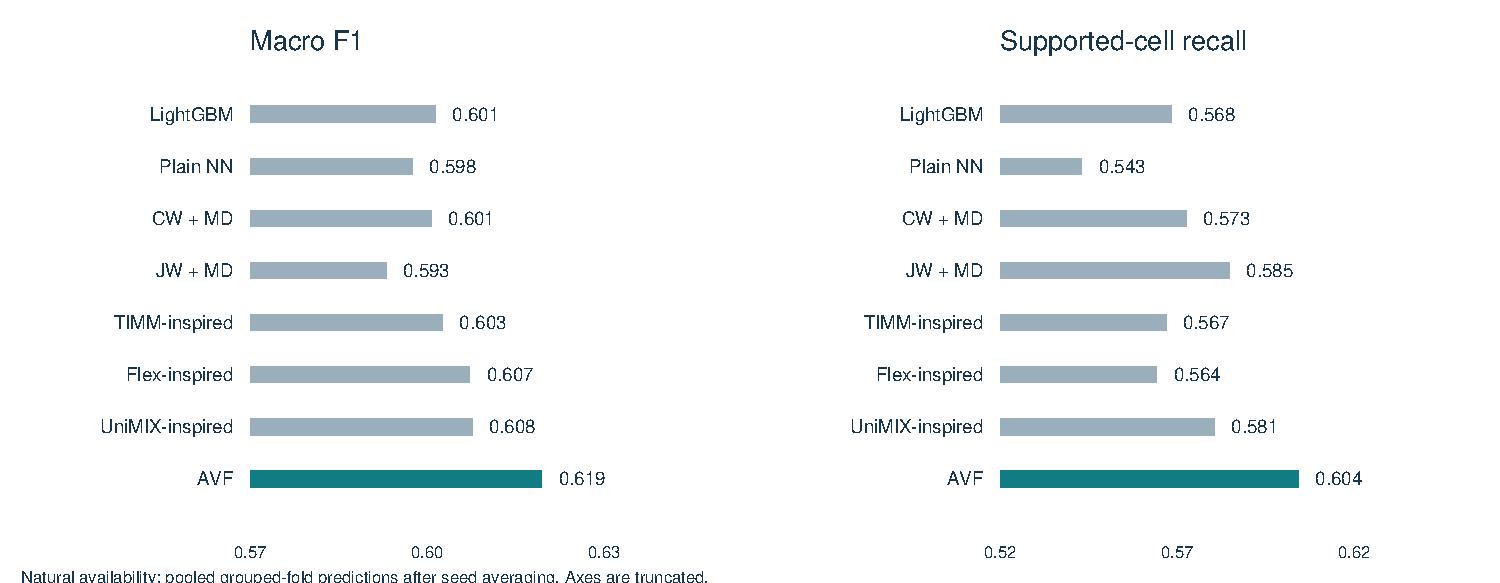
\includegraphics[width=\linewidth]{roi_performance}
\caption{Natural macro-F1 and SCR. The tree is a strong reference; joint balancing alone improves cell recall but does not dominate every metric. Axes are truncated to show differences and the figure does not display uncertainty.}\label{fig:performance}
\end{figure}

Table~\ref{tab:uncertainty} reports the original-sample differences alongside bootstrap intervals. The paired participant intervals support F1 and SCR gains for AVF, whereas the AUROC interval crosses zero. These intervals remain exploratory: they condition on the selected models and do not account for all selection or multiplicity.
\begin{table}[pos=!ht]
\caption{AVF minus seed-ensembled LightGBM. Point differences are replayed; 95\% percentile intervals are retained from the archived 1,000-resample participant bootstrap.}\label{tab:uncertainty}
\begin{tabular*}{\tblwidth}{@{} LCC @{}}\toprule
Metric & Point difference & 95\% interval \\ \midrule
Macro-AUROC & +0.00318 & [$-0.000052$, +0.00610] \\
Macro-F1 & +0.01803 & [+0.01021, +0.02559] \\
SCR & +0.03577 & [+0.02027, +0.05145] \\
Balanced accuracy & +0.02986 & Not estimated in this archived contrast \\
\bottomrule\end{tabular*}
\end{table}

\subsection{Factorial evidence and local comparator mechanisms}
Relative to the plain neural model, joint weighting with dropout raises SCR from 0.5431 to 0.5848 and balanced accuracy from 0.5984 to 0.6208, while AUROC falls from 0.7807 to 0.7783. Class weighting plus dropout instead yields macro-F1 0.6007 and SCR 0.5726. Thus joint weighting trades some discrimination and F1 for cell coverage; it is not a uniformly better loss. Fixed training-time logit adjustment gives the lowest AUROC and F1 among these arms, despite higher cell recall than the plain reference.

The three local comparator adaptations reach macro-F1 0.6027--0.6076. AVF has higher pooled natural F1 and SCR point estimates than all three. This ranking applies to the adaptations under the shared regional inputs and local training budget; it does not establish superiority over the published original systems.

\subsection{Member ablation and per-cell changes}
The archived member ablation in Table~\ref{tab:member} shows that fusion with a plain neural model already raises F1 to 0.6089 from the tree's 0.6014. Part of the gain thus comes from generic ensembling. Joint-plus-dropout fusion has the highest SCR and balanced accuracy among the tested members, while class-plus-dropout fusion has slightly higher AUROC and F1. AVF represents a cell-sensitive tradeoff, not a configuration that wins every metric. The ablation does not independently isolate any component's causal contribution.
\begin{table}[pos=!ht]
\caption{Tree fusion with alternative neural members. Archived rounded member-ablation values are shown to four decimals. Codes correspond to the factorial arms in Table~\ref{tab:natural}.}\label{tab:member}
\begin{tabular*}{\tblwidth}{@{} LCCCC @{}}\toprule
Neural member & AUROC & Macro F1 & BAcc & SCR \\ \midrule
none\_no\_drop & 0.7954 & 0.6089 & 0.6063 & 0.5699 \\
class\_no\_drop & 0.7970 & 0.6162 & 0.6181 & 0.5837 \\
joint\_no\_drop & 0.7964 & 0.6168 & 0.6204 & 0.5923 \\
none\_drop & 0.7968 & 0.6127 & 0.6087 & 0.5760 \\
class\_drop & 0.7977 & 0.6202 & 0.6235 & 0.5921 \\
joint\_drop & 0.7969 & 0.6194 & 0.6251 & 0.6043 \\
logitadj\_drop & 0.7964 & 0.6158 & 0.6220 & 0.5974 \\
\bottomrule\end{tabular*}
\end{table}
Across the 34 supported natural cells, 19 improve relative to LightGBM and the mean recall change is +0.03577 (Figure~\ref{fig:cells}). Several cells worsen, including common MCI patterns. The mean gain therefore does not establish improvement in every cell or in the worst cell. Sparse unsupported cells are outside the SCR estimate.
\begin{figure}[pos=!ht]
\centering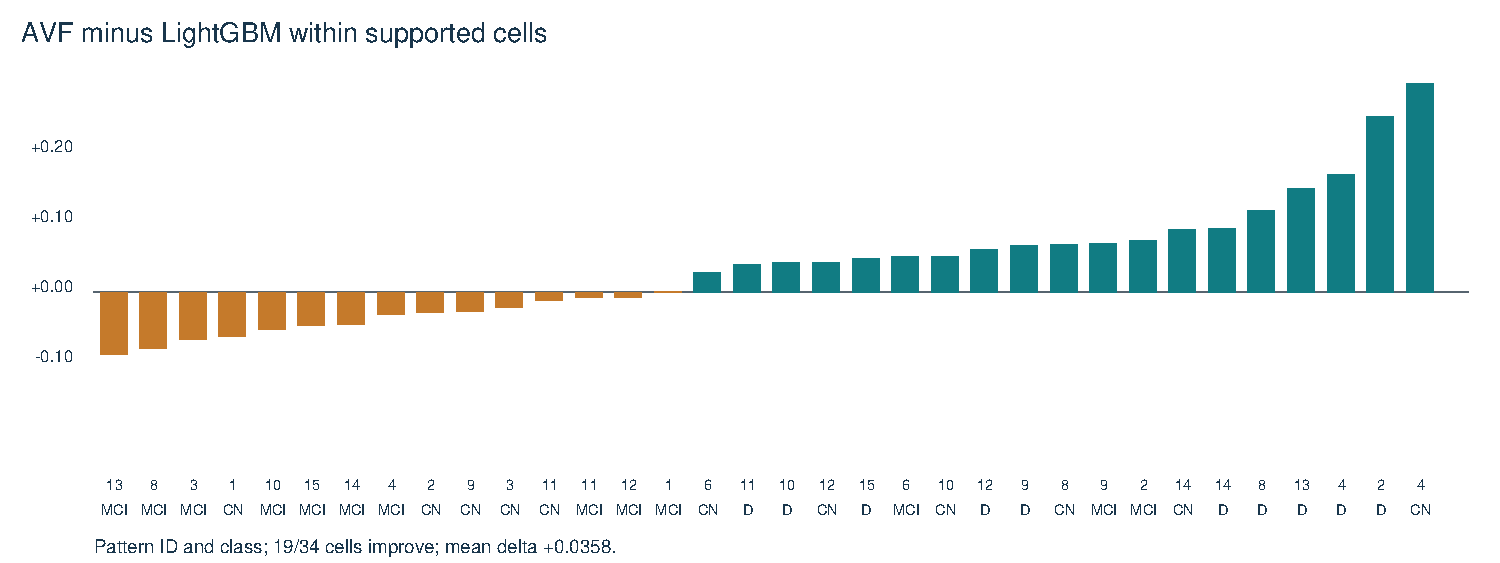
\includegraphics[width=\linewidth]{roi_cell_deltas}
\caption{AVF minus LightGBM recall in each supported class--pattern cell, ordered by difference. Pattern IDs use the four-bit encoding; D denotes dementia. Both improvements and regressions are retained.}\label{fig:cells}
\end{figure}
